
%butter
\textbf{Butterworth}
\begin{itemize}
    \item passband
    \begin{itemize}
        \item maximal flat
    \end{itemize}
    \item @cut-off frequency:
    \begin{itemize}
        \item -3dB attenuation
        \item -90 degree phaseshift
    \end{itemize}
    \item stopband 
    \begin{itemize}
        \item monotonic -40dB decline per decade
        \item approx. -37dB decline within fist decade
    \end{itemize} 
\end{itemize}

E.g.: Cut-off frequency is 10Hz. The bodeplot is shown in the figure \ref{fig:lp_butter} below.
\begin{figure}[h!]
  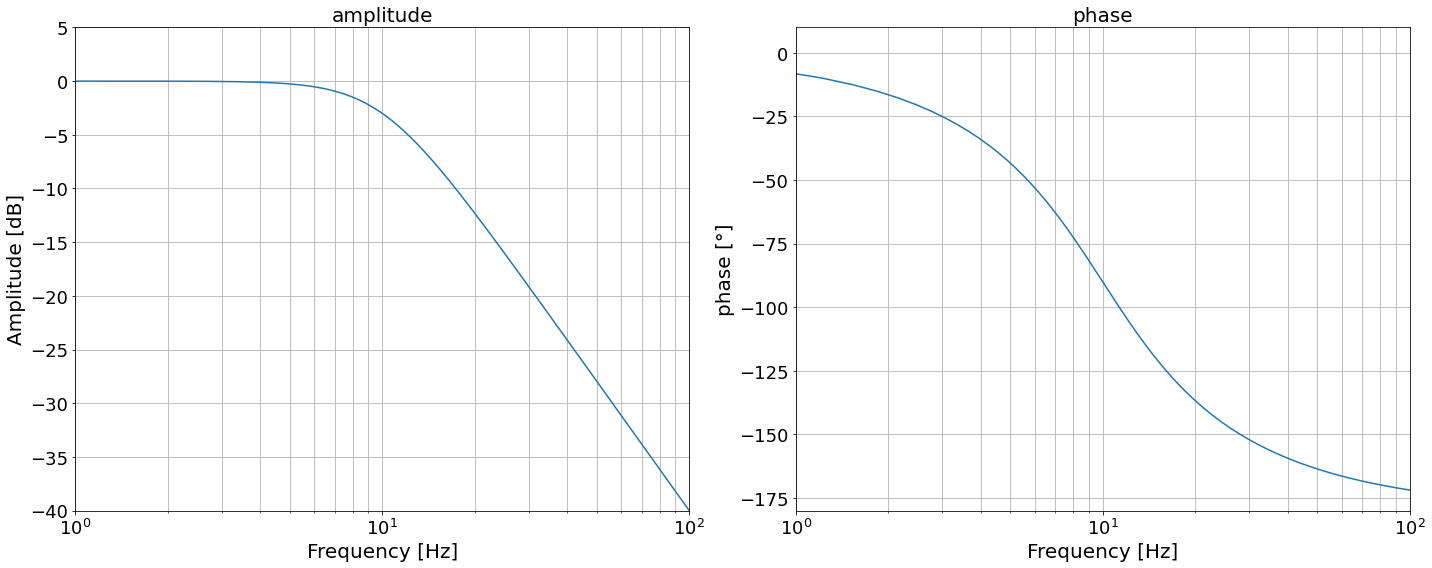
\includegraphics[width=0.75\linewidth]{lp_butter.png}
  \caption{Bodeplot Butterworth lowpass.}
  \label{fig:lp_butter}
\end{figure}
	
% Cheby1
\textbf{Chebyshev I}\\
\begin{itemize}
    \item passband:
    \begin{itemize}
        \item N/2=1 ripple in the passband.
        \item attenuation from 0 to $rp$ [dB].
    \end{itemize}
    \item @cut-off frequency: attenuation is bigger than or equal $rp$ [dB].
    \item stopband:
    \begin{itemize}
        \item monotonic -40dB decline per decade
    \end{itemize}
    \item Trade-off:
    \begin{itemize}
        \item the bigger passband ripple $rp$ is choosen, the steeper is the magnitude cut-off within the first decade in stopband 
        \item the bigger the passband ripple $rp$ is choosen, the bigger is the overall passband attenuation!
    \end{itemize}
\end{itemize}

E.g.: \\
Cut-off frequency is 10Hz.\\
The maximal ripple in the passband $rp$ must be given in [dB].\\
To show the mentioned trade-off, two bodelplots are shown. One with a small and one with a bigger $rp$.
The bodeplot is shown in the figures \ref{fig:lp_cheby1_1} and \ref{fig:lp_cheby1_2} below.
\begin{figure}[h!]
\centering
  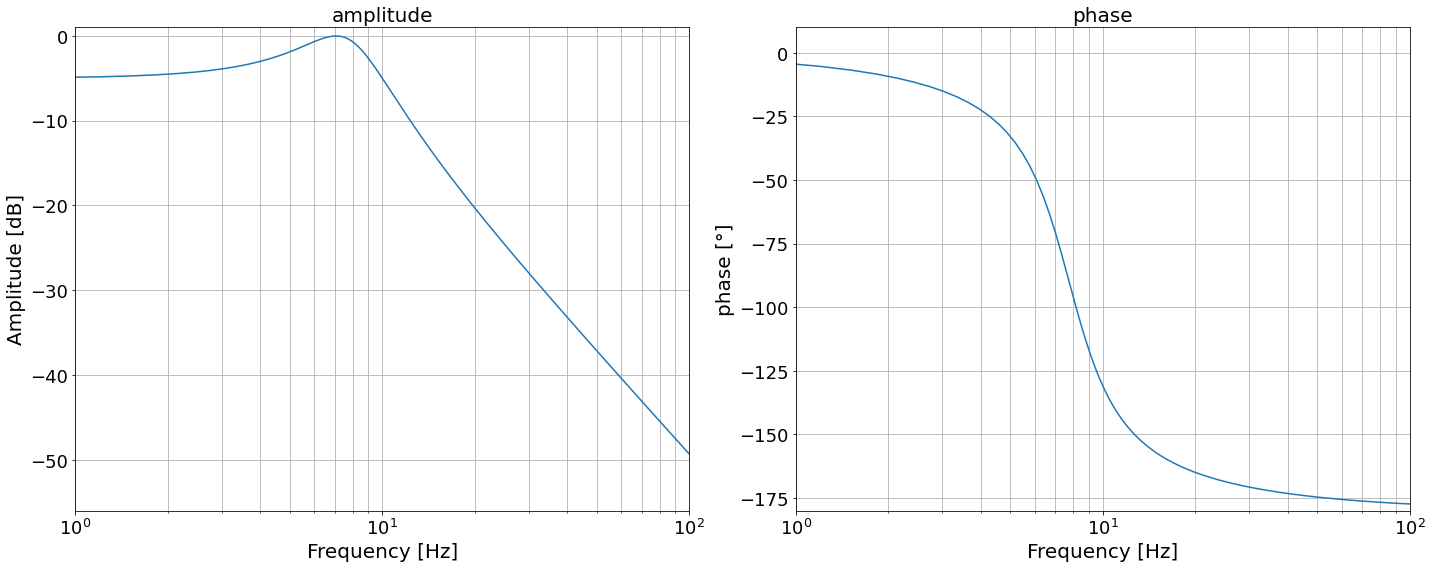
\includegraphics[width=0.75\linewidth]{lp_cheby1_5dB.png}
  \caption{Bodeplot Chebyshev I lowpass. $rp=5$dB}
  \label{fig:lp_cheby1_1}
\end{figure}

\begin{figure}[h!]
\centering
  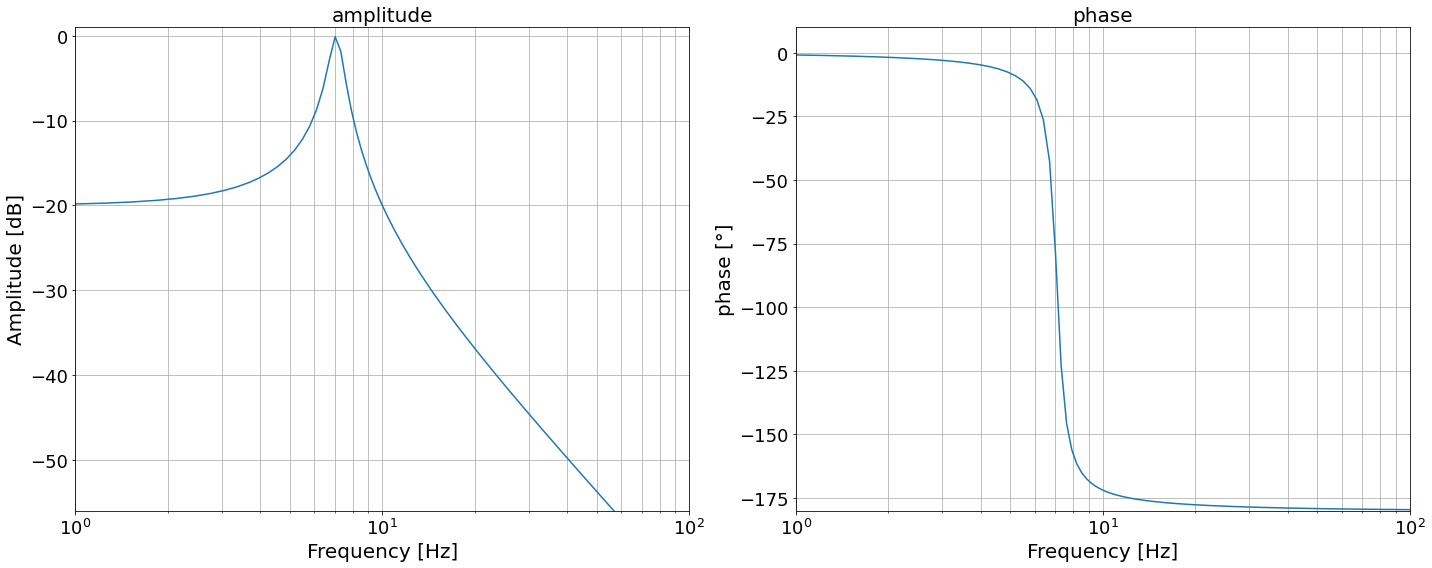
\includegraphics[width=.75\linewidth]{lp_cheby1_20dB.png}
  \caption{Bodeplot Chebyshev I lowpass. $rp=20$dB}
  \label{fig:lp_cheby1_2}
\end{figure}

% Cheby2
\textbf{Chebyshev II}\\
Also known as inverse Chebyshev filter.\\
\begin{itemize}
    \item passband
    \begin{itemize}
         \item flat, no ripples 
    \end{itemize}
    \item @cut-off frequency: attenuation is $rs$ [dB].
    \item stopband
    \begin{itemize}
        \item N/2=1 ripple in the stopband
        \item attenuation is smaller than or equal $rs$ [dB].
    \end{itemize}
    \item Trade-off:
    \begin{itemize}
        \item the lower $rs$ is choosen, the sharper is the magnitude cut-off
        \item the lower $rs$ is choosen, the lower is the over all stopband attenuation
    \end{itemize}
\end{itemize}

E.g.: \\
Cut-off frequency is 10Hz.\\
The maximal ripple in the stopband $rs$ must be given in [dB].\\
To show the mentioned trade-off, two bodelplots are shown. One with a small and one with a bigger $rs$.
The bodeplot is shown in the figures \ref{fig:lp_cheby2_1} and \ref{fig:lp_cheby2_2} below.
\begin{figure}[h!]
\centering
  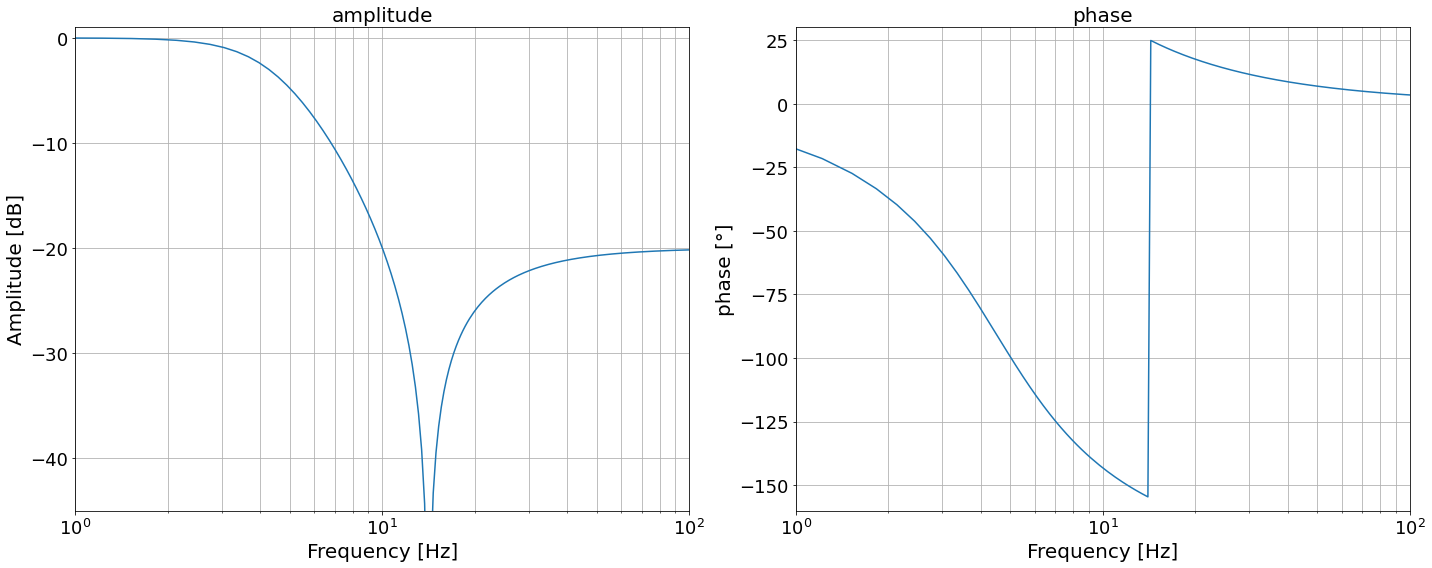
\includegraphics[width=.75\linewidth]{lp_cheby2_20dB.png}
  \caption{Bodeplot Chebyshev II lowpass. $rs=20$dB}
  \label{fig:lp_cheby2_1}
\end{figure}

\begin{figure}[h!]
\centering
  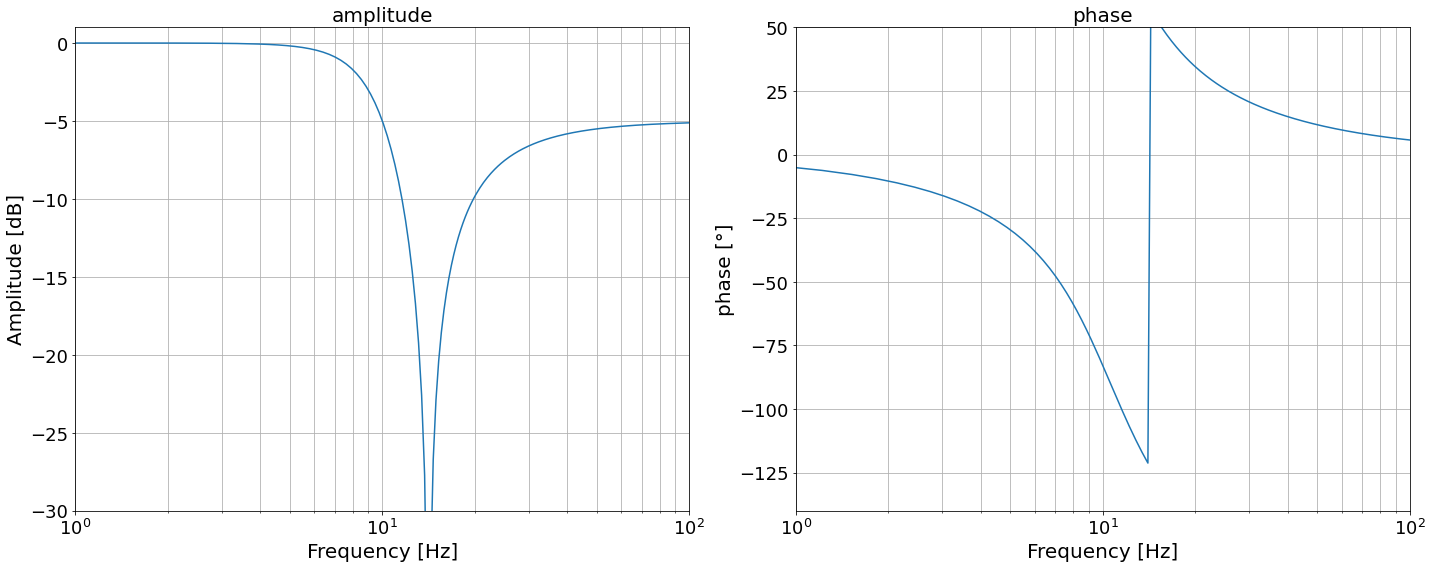
\includegraphics[width=.75\linewidth]{lp_cheby2_5dB.png}
  \caption{Bodeplot Chebyshev II lowpass. $rs=5$dB}
  \label{fig:lp_cheby2_2}
\end{figure}

%bessel
\textbf{Bessel}\\
\begin{itemize}
    \item passband
    \begin{itemize}
        \item constant group-delay in passband.
		\item least sharp magnitude roll-off.
    \end{itemize}
    \item @cut-off frequency:
    \begin{itemize}
        \item approx. -1.6 dB attenuation
        \item approx. -56 degree phaseshift
    \end{itemize}
    \item stopband 
    \begin{itemize}
        \item monotonic -40dB decline per decade
        \item approx. -30dB decline within first decade
    \end{itemize} 
\end{itemize}

E.g.: \\
Cut-off frequency is 10Hz.\\
The bodeplot is shown in the figure \ref{fig:lp_bessel} below.
\begin{figure}[h!]
  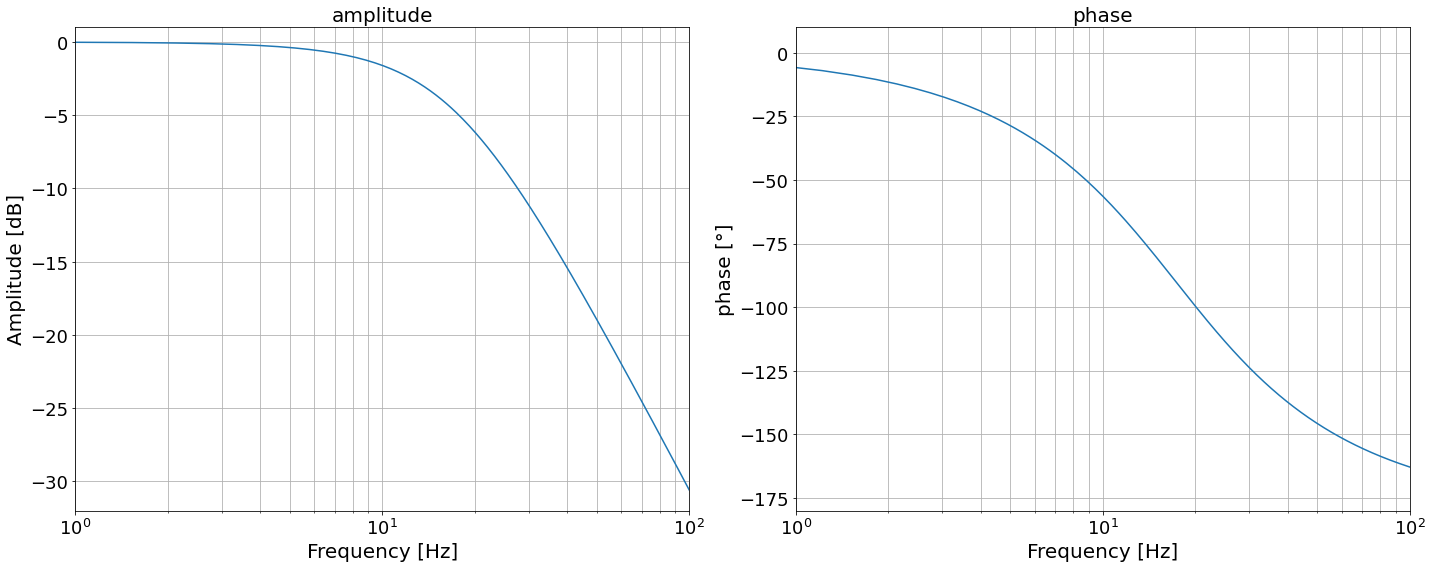
\includegraphics[width=.75\linewidth]{lp_bessel.png}
  \caption{Bodeplot Bessel lowpass.}
  \label{fig:lp_bessel}
\end{figure}